\documentclass[english,10pt,a4paper]{article}
\usepackage{tcolorbox}
\usepackage{ulem} %math
\usepackage{amsmath}
\usepackage{amsfonts}
\usepackage{amssymb}
\usepackage{graphicx}
\usepackage{enumerate}


%Create a box for theorems
%\begin{theo}[titel] %optional
%tekst
%\end{theo}
\newenvironment{theo}[1][Vigtigt]{%
\begin{tcolorbox}[colback=green!5,colframe=green!40!black,title=\textbf{#1}]
}{%
\end{tcolorbox}
}




%Create a square matrix
%\begin{ArgMat}{2}
%21 & 22 & 23 \\  
%a & b & c
%\end{ArgMat}
%
% Info: http://tex.stackexchange.com/questions/2233/whats-the-best-way-make-an-augmented-coefficient-matrix
%
\newenvironment{ArgMat}{%
$
  \left[\begin{array}{@{}*{100}{r}r@{}}
}{%
  \end{array}\right]
  $
}

\newenvironment{deter}{%
$
  \left|\begin{array}{@{}*{100}{r}r@{}}
}{%
  \end{array}\right|
  $
}


%Create multiple lines with holes
%\begin{SysEqu}
%x_1 && &- &5x_3 &+ &2x_4=& 1 \\
%x_1 &+ &x_2 &+ &x_3 && =& 4 \\
%&&&&&&0 =& 0
%\end{SysEqu}
\newenvironment{SysEqu}{%
$  \setlength\arraycolsep{0.1em}
  \begin{array}{@{}*{100}{r}r@{}}
}{%
  \end{array}$
}

%Create solution for x_1, x_n...
%\begin{solu}
%x_1 &= d \\
%x_2 &= e \\
%x_3 &= s
%\end{solu}
\newenvironment{solu}{%
$
  \setlength\arraycolsep{0.1em}
  \left\{\begin{array}{@{}*{100}{r}r@{}}
}{%
  \end{array}\right.
$
}

\usepackage{lastpage}


\newcommand{\HRule}{\rule{\linewidth}{0.8mm}}

%Tekst i fotter
\newcommand{\footerText}{\thepage\xspace /\pageref{LastPage}}
\newcommand{\ProjectName}{433 MHz styring af AeroQuad}


\chapterstyle{hangnum}




\nouppercaseheads
\makepagestyle{mystyle} 

\makeevenhead{mystyle}{}{\\ \leftmark}{} 
\makeoddhead{mystyle}{}{\\ \leftmark}{} 
\makeevenfoot{mystyle}{}{\footerText}{} 
\makeoddfoot{mystyle}{}{\footerText}{} 
\makeatletter
\makepsmarks{mystyle}{% Overskriften på sidehovedet
  \createmark{chapter}{left}{shownumber}{\@chapapp\ }{.\ }} 
\makeatother
\makefootrule{mystyle}{\textwidth}{\normalrulethickness}{0.4pt}
\makeheadrule{mystyle}{\textwidth}{\normalrulethickness}

\makepagestyle{plain}
\makeevenhead{plain}{}{}{}
\makeoddhead{plain}{}{}{}
\makeevenfoot{plain}{}{\footerText}{}
\makeoddfoot{plain}{}{\footerText}{}
\makefootrule{plain}{\textwidth}{\normalrulethickness}{0.4pt}

\pagestyle{mystyle}

%%----------------------------------------------------------------------
%
%%Redefining chapter style
%%\renewcommand\chapterheadstart{\vspace*{\beforechapskip}}
%\renewcommand\chapterheadstart{\vspace*{10pt}}
%\renewcommand\printchaptername{\chapnamefont }%\@chapapp}
%\renewcommand\chapternamenum{\space}
%\renewcommand\printchapternum{\chapnumfont \thechapter}
%\renewcommand\afterchapternum{\space: }%\par\nobreak\vskip \midchapskip}
%\renewcommand\printchapternonum{}
%\renewcommand\printchaptertitle[1]{\chaptitlefont #1}
\setlength{\beforechapskip}{0pt} 
\setlength{\afterchapskip}{0pt} 
%\setlength{\voffset}{0pt} 
\setlength{\headsep}{25pt}
%\setlength{\topmargin}{35pt}
%%\setlength{\headheight}{102pt}
%\setlength{\textheight}{302pt}
\renewcommand\afterchaptertitle{\par\nobreak\vskip \afterchapskip}
%%----------------------------------------------------------------------




%Sidehoved og -fod pakke
%Margin
\usepackage[left=2cm,right=2cm,top=2.5cm,bottom=2cm]{geometry}
\usepackage{lastpage}



%%URL kommandoer og sidetal farve
%%Kaldes med \url{www...}
%\usepackage{color} %Skal også bruges
\usepackage{hyperref}
\hypersetup{ 
	colorlinks	= true, 	% false: boxed links; true: colored links
    urlcolor	= blue,		% color of external links
    linkcolor	= black, 	% color of page numbers
    citecolor	= blue,
}



%Mellemrum mellem linjerne    
\linespread{1.5}


%Seperated files
%--------------------------------------------------
%Opret filer således:
%\documentclass[Navn-på-hovedfil]{subfiles}
%\begin{document}
% Indmad
%\end{document}
%
% I hovedfil inkluderes således:
% \subfile{navn-på-subfil}
%--------------------------------------------------
\usepackage{subfiles}

%Prevent wierd placement of figures
%\usepackage[section]{placeins}

%Standard sti at søge efter billeder
%--------------------------------------------------
%\begin{figure}[hbtp]
%\centering
%\includegraphics[scale=1]{filnavn-for-png}
%\caption{Titel}
%\label{fig:referenceNavn}
%\end{figure}
%--------------------------------------------------
\usepackage{graphicx}
\usepackage{subcaption}
\usepackage{float}
\graphicspath{{../Figures/}}

%Speciel skrift for enkelt linje kode
%--------------------------------------------------
%Udskriver med fonten 'Courier'
%Mere info her: http://tex.stackexchange.com/questions/25249/how-do-i-use-a-particular-font-for-a-small-section-of-text-in-my-document
%Eksempel: Funktionen \code{void Hello()} giver et output
%--------------------------------------------------
\newcommand{\code}[1]{{\fontfamily{pcr}\selectfont #1}}


% Følgende er til koder.
%----------------------------------------------------------
%\begin{lstlisting}[caption=Overskrift på boks, style=Code-C++, label=lst:referenceLabel]
%public void hello(){}
%\end{lstlisting}
%----------------------------------------------------------

%Exstra space
\usepackage{xspace}
%Navn på bokse efterfulgt af \xspace (hvis det skal være mellemrum
%gives det med denne udvidelse. Ellers ingen mellemrum.
\newcommand{\codeTitle}{Kodeudsnit\xspace}

%Pakker der skal bruges til lstlisting
\usepackage{listings}
\usepackage{color}
\usepackage{textcomp}
\definecolor{listinggray}{gray}{0.9}
\definecolor{lbcolor}{rgb}{0.9,0.9,0.9}
\renewcommand{\lstlistingname}{\codeTitle}
\lstdefinestyle{Code}
{
	keywordstyle	= \bfseries\ttfamily\color[rgb]{0,0,1},
	identifierstyle	= \ttfamily,
	commentstyle	= \color[rgb]{0.133,0.545,0.133},
	stringstyle		= \ttfamily\color[rgb]{0.627,0.126,0.941},
	showstringspaces= false,
	basicstyle		= \small,
	numberstyle		= \footnotesize,
%	numbers			= left, % Tal? Udkommenter hvis ikke
	stepnumber		= 2,
	numbersep		= 6pt,
	tabsize			= 2,
	breaklines		= true,
	prebreak 		= \raisebox{0ex}[0ex][0ex]{\ensuremath{\hookleftarrow}},
	breakatwhitespace= false,
%	aboveskip		= {1.5\baselineskip},
  	columns			= fixed,
  	upquote			= true,
  	extendedchars	= true,
 	backgroundcolor = \color{lbcolor},
	lineskip		= 1pt,
%	xleftmargin		= 17pt,
%	framexleftmargin= 17pt,
	framexrightmargin	= 0pt, %6pt
%	framexbottommargin	= 4pt,
}

%Bredde der bruges til indryk
%Den skal være 6 pt mindre
\usepackage{calc}
\newlength{\mywidth}
\setlength{\mywidth}{\textwidth-6pt}


% Forskellige styles for forskellige kodetyper
\usepackage{caption}
\DeclareCaptionFont{white}{\color{white}}
\DeclareCaptionFormat{listing}%
{\colorbox[cmyk]{0.43, 0.35, 0.35,0.35}{\parbox{\mywidth}{\hspace{5pt}#1#2#3}}}
\captionsetup[lstlisting]
{
	format			= listing,
	labelfont		= white,
	textfont		= white, 
	singlelinecheck	= false, 
	width			= \mywidth,
	margin			= 0pt, 
	font			= {bf,footnotesize}
}

\lstdefinestyle{Code-C} {language=C, style=Code}
\lstdefinestyle{Code-Java} {language=Java, style=Code}
\lstdefinestyle{Code-C++} {language=[Visual]C++, style=Code}
\lstdefinestyle{Code-VHDL} {language=VHDL, style=Code}
\lstdefinestyle{Code-Bash} {language=Bash, style=Code}

%Text typesetting
%--------------------------------------------------------
%\usepackage{baskervald}
\usepackage{lmodern}
\usepackage[T1]{fontenc}              
\usepackage[utf8]{inputenc}         
\usepackage[english]{babel}       

\setlength{\parindent}{0pt}
\nonzeroparskip

%\setaftersubsecskip{1sp}
%\setaftersubsubsecskip{1sp}
 


%Dybde på indholdsfortegnelse
%----------------------------------------------------------
%Chapter, section, subsection, subsubsection
%----------------------------------------------------------
\setcounter{secnumdepth}{3}
\setcounter{tocdepth}{3}


%Tables
%----------------------------------------------------------
\usepackage{tabularx}
\usepackage{array}
\usepackage{multirow} 
\usepackage{multicol} 
\usepackage{booktabs}
\usepackage{wrapfig}
\renewcommand{\arraystretch}{1.5}



%Misc
%----------------------------------------------------------
\usepackage{cite}
\usepackage{appendix}
\usepackage{amssymb}
\usepackage{url,ragged2e}
\usepackage{enumerate}
\usepackage{amsmath} %Math bibliotek


\usepackage{longtable}


\title{Exam quistions}
\author{10893, Rasmus Bækgaard}
\date{August 30th, 2013}
\begin{document}
\maketitle

\section{Set}

\begin{theo}[Symbols] 

\begin{itemize}
\item \textbf{N} -- natural number (positive integers)
\item \textbf{Z} -- integers -- hele tal.
\item \textbf{Q} -- rational numbers -- $\dfrac{m}{n}$ where $m, n \in \mathbb{Z}$
\item \textbf{I} -- irrational numbers -- like $\sqrt{2}, \pi$
\item \textbf{R} -- real numbers -- Everything with and without comma.
\item \textbf{C} -- complex numbers -- $a+b\cdot i$
\item $\emptyset$ -- Empty set -- nothing
\end{itemize}

\end{theo}

\begin{theo}[Cardinal number / cardinality] 
The amount of elements in a set:\\
$|S| = \{ 2, -3, \emptyset\} = 3$

\end{theo}




\subsection{Subset}
\begin{itemize}
\item A set within a set: $S=\{a, b, c\}, T = \{a, b \}, U= \{ a, b, c\}, V=\{c\}$
\item Can be written as $T \subseteq S$
	\begin{itemize}
	\item Pronounced \textit{T is a \textbf{proper} subset of S}
	\end{itemize}
\item Can be written as $S \subseteq U$
	\begin{itemize}
	\item Pronounced \textit{S is a subset of U}
	\end{itemize}
	
\item If a set is not in another set it's written as $T \not \subseteq V$
\end{itemize}


\begin{theo}[Intervals] 
\begin{itemize}
\item Open, $(a,b) = \{ x \in \mathbb{R}: a < x < b \}$
\item Closed, $[a,b] = \{ x \in \mathbb{R}: a \leq x \leq b \}$
\item Half open, $[a,b) = \{ x \in \mathbb{R}: a \leq x < b \}$
\item Half closed, $(a,b] = \{ x \in \mathbb{R}: a < x \leq b \}$
\end{itemize}
\end{theo}


\begin{theo}[Power set] 
\begin{itemize}
\item A combination of all elements as \textbf{subsets}:
\item[] $A=\emptyset, B= \{a,b\}, C=\{1,2,3\}$
\item $\mathcal{P}(A) = \{\emptyset\} $
\item $\mathcal{P}(B) = \{\emptyset, \{a\}, \{b\}, \{a,b\} \}$
\item $\mathcal{P}(C) = \{\emptyset, \{1\}, \{2\}, \{3\}, \{1,2\}, \{1,3\}, \{2, 3\}, \{1,2,3\} \}$
\item Cardinality: $|\mathcal{P}(A)| = 2^{|A|}$
\item $\mathcal{P}(set) = \{subset : subset \subseteq set\}$
\end{itemize}
\end{theo}



\subsection{Set operations}
\begin{theo}[Union] 
\begin{itemize}
\item Means "in total"
\item Written as $A \cup B$
\item[] \includegraphics[scale=1]{union} 
\item SQL: \code{SELECT A, B IN Sets}
\end{itemize}

\end{theo}



\begin{theo}[Intersection] 
\begin{itemize}
\item Means "in common"
\item Written as $A \cap B$
\item[] 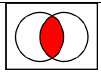
\includegraphics[scale=1]{Intersection} 
\item If nothing is in common it's called \textbf{disjoint} and written $A \cap B = \emptyset$
\item Can be written as $A \cap B = \{ x \in A \vee x \in B : x \in A \wedge x \in B \}$
\item SQL: \\\code{SELECT A, B \\ FROM SetA \\INNER JOIN SetB \\ON A.a = b.a}
\end{itemize}

\end{theo}



\begin{theo}[Difference] 
\begin{itemize}
\item Means "What does A have which B does not"
\item Written as $A - B$
\item[] 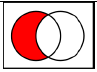
\includegraphics[scale=1]{Difference} 
\item Can also be written as $A \setminus B $
\item SQL: \\\code{SELECT A, B \\ FROM SetA \\INNER JOIN SetB \\ON A.a = b.a}
\end{itemize}

\end{theo}





\section{Proofs}


\begin{theo}[Trivial proof] 
\begin{itemize}
\item Something that is true -- no need to prove it.
\item Let $n \in \mathbb{Z}$. If $n^3 > 0$ then 3 is odd
\end{itemize}
\end{theo}



\begin{theo}[Vacouos proof] 
\begin{itemize}
\item If something is always proven wrong
\item Let $n \in \mathbb{Z}$. If \textbf{3 is even}, then $n^3 > 0$
\item[] Clearly wrong!
\end{itemize}
\end{theo}



\begin{theo}[Direct proof] 
\begin{itemize}
\item Show only what needs to be shown
\item $\forall x \in S, P(x) \Rightarrow Q(x)$
\item[] Show only that this is true and where it is false, e.g. show truth table.
\item Is shown from lemmas and other proves.
\end{itemize}
\end{theo}



\begin{theo}[Indirect proof / proof by contrapositive] 
\begin{itemize}
\item Reverse the result an means.
\item Let $x \in S$. If $Q(x)$, then $P(x) \Rightarrow$
\item[] Let $x \in S$. If $\neg Q(x)$, then $\neg P(x)$
\end{itemize}
\end{theo}



\begin{theo}[Proof by cases] 
\begin{itemize}
\item Do subcases and show they span the result.
\item Case 1: $n$ is even (U). Case 2: $n$ is odd (L). $\mathbb{Z} = U \cup L $
\item Case 1: $n>0$ (U). Case 2: $n<0$ (L). $\mathbb{Z} = U \cup L$
\item \textbf{Show $P \Leftrightarrow Q$ example}
\end{itemize}
\end{theo}






\end{document}